% This version of CVPR template is provided by Ming-Ming Cheng.
% Please leave an issue if you found a bug:
% https://github.com/MCG-NKU/CVPR_Template.

\documentclass[final]{cvpr}

\usepackage{times}
\usepackage{epsfig}
\usepackage{graphicx}
\usepackage{amsmath}
\usepackage{amssymb}
\usepackage{float}
\usepackage{overpic}
\usepackage{caption}
\usepackage{booktabs}
\usepackage{tikz}
\usetikzlibrary{arrows.meta, positioning, fit, backgrounds}

\usepackage[pagebackref=true,breaklinks=true,colorlinks,bookmarks=false]{hyperref}

\begin{document}

%%%%%%%%% TITLE
\title{VulnScout: An Always-Current, Tool-Grounded Assistant for Vulnerability Triage}

\author{Yuanhao Cao\\
MS in Information Systems\\
Northeastern University\\
cao.yuanh@northeastern.edu
}

\twocolumn[{
    \renewcommand\twocolumn[1][]{#1}%
    \maketitle
    \begin{center}
      \centering
      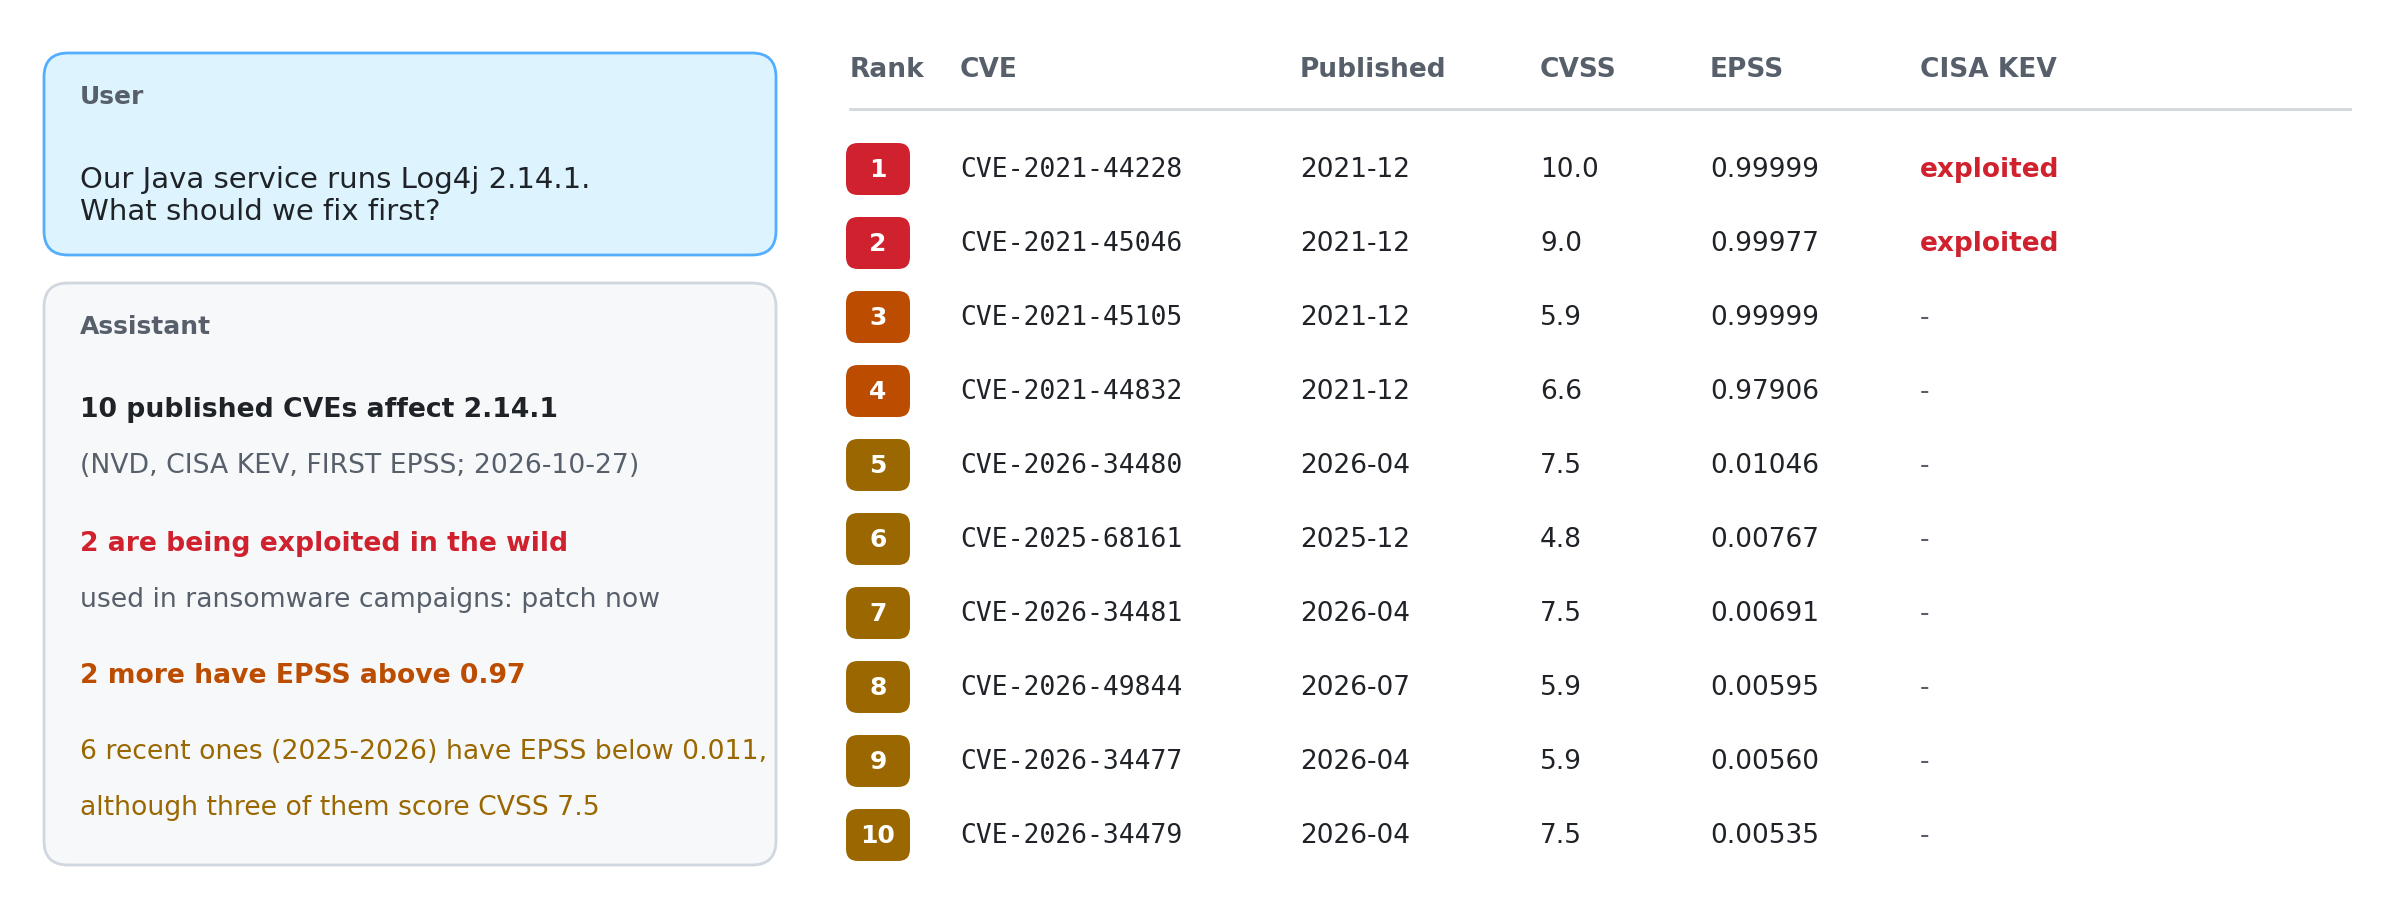
\includegraphics[width=\textwidth]{fig/cover.png}
      \captionof{figure}{What VulnScout is meant to produce, using real data. For ``Log4j 2.14.1'', the NVD API returns 10 CVEs that affect this version; we ranked them with the CISA Known Exploited Vulnerabilities (KEV) catalog and FIRST EPSS exploit probabilities, all queried on 2026-10-27. Six of the ten were published in 2025--2026, after many LLMs' training cutoffs, and ranking by CVSS alone would place three low-probability 7.5-score CVEs above two older CVEs that have EPSS above 0.97.}
      \label{fig_teaser}
    \end{center}
}]

%%%%%%%%% BODY TEXT
\section*{Abstract}
Thousands of software vulnerabilities are disclosed every week, and teams without dedicated security staff struggle to answer two questions: \emph{does this vulnerability affect the exact version I run}, and \emph{what should I fix first?} General-purpose LLMs answer from a frozen training snapshot and often guess version ranges. We propose VulnScout, a conversational assistant that takes a natural-language description of a software stack, retrieves current vulnerability records from public sources (NVD, CVE records, OSV), decides affected versions with a deterministic, provenance-tracked resolver instead of the LLM, ranks findings by real-world exploitation evidence (CISA KEV, EPSS) rather than severity alone, and returns cited explanations and remediation advice. The target users are developers and IT operators who need fast, trustworthy triage.

%-------------------------------------------------------------------------
\section{Introduction}

\subsection{Target market}
Vulnerability management is a core operational need for every organization that runs software, and its volume keeps growing. In the seven days before 2026-10-27 alone, the National Vulnerability Database (NVD) published 4,433 new CVE records~\cite{nvd}, more than 600 per day. Severity scores do not settle what to patch first: CVSS describes how bad a vulnerability \emph{could} be, while only a small fraction of vulnerabilities is ever exploited. This gap motivated data-driven signals such as the Exploit Prediction Scoring System (EPSS)~\cite{jacobs2019epss,jacobs2023epss} and CISA's Known Exploited Vulnerabilities (KEV) catalog~\cite{cisakev}, which listed 1,760 vulnerabilities on the same date.

The data itself is also becoming harder to use. In a sample of 2,000 CVEs published in that week, only 23.0\% carried NVD's machine-readable list of affected products and versions (CPE configurations), and 52\% were still ``Awaiting Analysis''. The vendor-submitted CVE records~\cite{cvelistv5} usually do state affected versions (all 40 records in a random sample of the remaining CVEs did), but in inconsistent formats, for example a single string ``26.7.0-26.7.1'' instead of structured bounds.

\subsection{Target users}
VulnScout targets developers, DevOps engineers and IT operators in small and mid-sized organizations, and students running their own services, who have no dedicated security team. Their typical questions are informal, such as ``our Java service still runs Log4j 2.14.1, what should we fix first?'', and they need answers that are (1) \emph{current}, covering vulnerabilities disclosed this week; (2) \emph{version-exact}, stating whether their specific version is affected; (3) \emph{prioritized} by real-world risk; and (4) \emph{verifiable}, with links to official records.

\subsection{Problem}
General-purpose LLMs fail all four requirements in characteristic ways. Their knowledge stops at a training cutoff, while for Log4j 2.14.1 alone six of the ten affecting CVEs were published in 2025--2026 (Figure~\ref{fig_teaser}). Their answers about version ranges are generated rather than computed: the NVD record of Log4Shell (CVE-2021-44228) lists 396 affected-product entries, each with its own version bounds and exclusions. They tend to rank by severity, and they can fabricate plausible identifiers, a failure mode already documented for software packages~\cite{spracklen2025package}. Existing scanners solve version matching for structured inputs but do not offer conversational, explained triage (Section~\ref{sec:related}).

%-------------------------------------------------------------------------
\section{Related Work}
\label{sec:related}

\textbf{Vulnerability data and prioritization.} NVD~\cite{nvd} enriches CVE records with CVSS scores, weakness types (CWE) and CPE configurations; the CVE Program publishes the original CNA-submitted records in CVE JSON 5~\cite{cvelistv5}; OSV~\cite{osv} provides package-ecosystem version ranges for open-source software. For prioritization, EPSS~\cite{jacobs2019epss} estimates the probability that a vulnerability will be exploited in the next 30 days, and its later versions use community data to improve over severity-based strategies, which are poor predictors of exploitation~\cite{jacobs2023epss}. CISA KEV~\cite{cisakev} records vulnerabilities with confirmed exploitation. VulnScout builds on these sources rather than replacing them.

\textbf{Software composition analysis (SCA).} Scanners such as Trivy~\cite{trivy}, Grype~\cite{grype}, OSV-Scanner~\cite{osvscanner} and Dependabot~\cite{dependabot} match the dependencies in manifests, lock files or container images against vulnerability databases. They are mature and accurate for structured inputs, but they expect those inputs, return lists rather than answers to questions, and are not designed for free-form descriptions (``the Cisco router in our office'') or follow-up questions. VulnScout is complementary: it can use the same databases, while adding natural-language understanding, explanation and dialogue.

\textbf{LLMs in cybersecurity.} A systematic review by Xu \etal~\cite{xu2024llmsecurity} surveys LLM applications across security tasks. CyberMetric~\cite{tihanyi2024cybermetric} evaluates general cybersecurity knowledge with multiple-choice questions, and CTIBench~\cite{alam2024ctibench} evaluates cyber-threat-intelligence tasks motivated by concerns about reliability and hallucination. These benchmarks measure what a model \emph{knows}; VulnScout instead keeps facts outside the model. Open-source LLM prototypes over NVD exist~\cite{nvdchatbot,cvellmdataset}, but we did not find one that evaluates version correctness or freshness systematically.

\textbf{Retrieval, tool use and freshness.} Retrieval-augmented generation (RAG)~\cite{lewis2020rag} conditions generation on retrieved documents, and ReAct~\cite{yao2023react} and Toolformer~\cite{schick2023toolformer} let models call external tools during reasoning. FreshQA~\cite{vu2023freshllms} and RealTime QA~\cite{kasai2022realtimeqa} show that static LLMs fail on fast-changing knowledge and that search augmentation helps. VulnScout applies these ideas to a domain where freshness is measurable (publication dates) and where some decisions, such as version comparison, should be computed rather than generated.

\begin{figure*}[t]
\centering
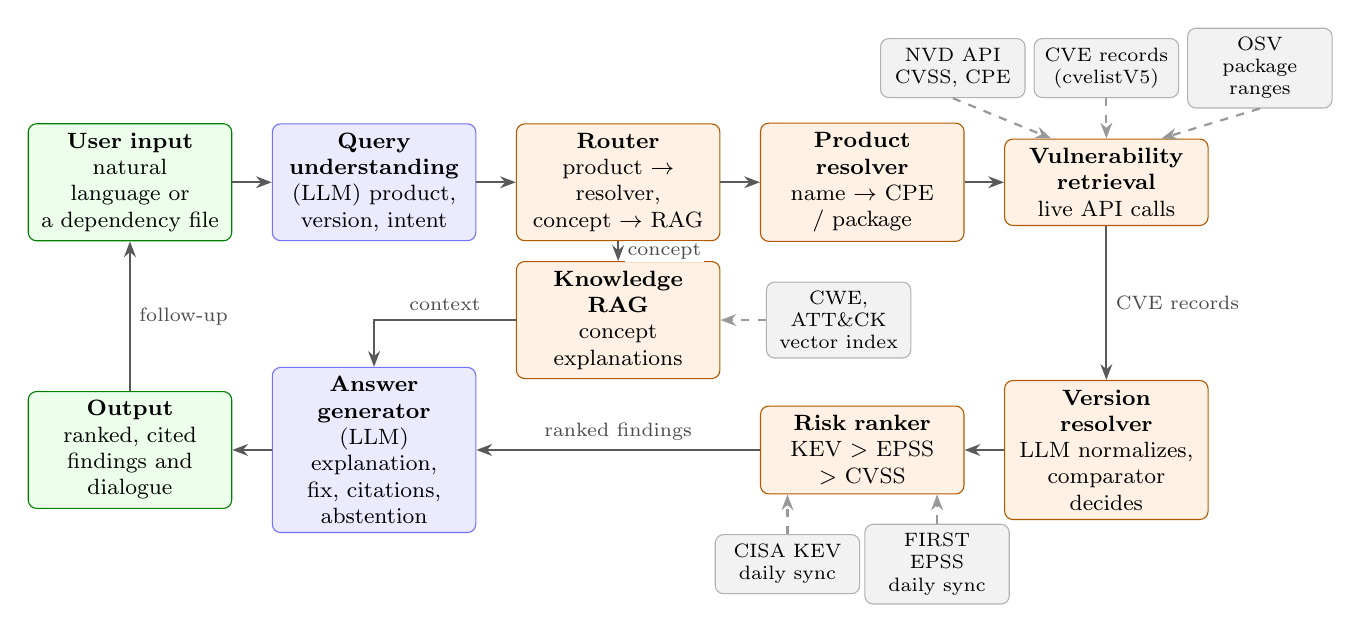
\begin{tikzpicture}[
    box/.style={draw=black!60, rounded corners=3pt, align=center, font=\footnotesize,
                minimum height=1.05cm, text width=2.35cm, fill=white,
                execute at begin node={\hyphenpenalty=10000\relax}},
    llm/.style={box, fill=blue!8, draw=blue!55},
    tool/.style={box, fill=orange!10, draw=orange!70!black},
    data/.style={box, fill=gray!10, draw=gray!60, text width=1.6cm, minimum height=0.75cm, font=\scriptsize},
    io/.style={box, fill=green!8, draw=green!50!black},
    arr/.style={-{Stealth[length=2mm]}, thick, black!65},
    darr/.style={-{Stealth[length=2mm]}, thick, black!40, dashed},
    lbl/.style={font=\scriptsize, black!70, fill=white, inner sep=1pt},
]
% row 1: question understanding and retrieval
\node[io]   (user)     at (0,0)     {\textbf{User input}\\natural language or a dependency file};
\node[llm]  (parse)    at (3.1,0)   {\textbf{Query understanding}\\(LLM) product, version, intent};
\node[tool] (router)   at (6.2,0)   {\textbf{Router}\\product $\rightarrow$ resolver, concept $\rightarrow$ RAG};
\node[tool] (resolve)  at (9.3,0)   {\textbf{Product resolver}\\name $\rightarrow$ CPE / package};
\node[tool] (fetch)    at (12.4,0)  {\textbf{Vulnerability retrieval}\\live API calls};
% middle: knowledge RAG for conceptual questions
\node[tool] (rag)      at (6.2,-1.75) {\textbf{Knowledge RAG}\\concept explanations};
% row 2: resolution, ranking and answer
\node[io]   (out)      at (0,-3.4)    {\textbf{Output}\\ranked, cited findings and dialogue};
\node[llm]  (answer)   at (3.1,-3.4)  {\textbf{Answer generator}\\(LLM) explanation, fix, citations, abstention};
\node[tool] (rank)     at (9.3,-3.4)  {\textbf{Risk ranker}\\KEV $>$ EPSS $>$ CVSS};
\node[tool] (version)  at (12.4,-3.4) {\textbf{Version resolver}\\LLM normalizes, comparator decides};
% external data sources
\node[data] (nvd)  at (10.45,1.45) {NVD API\\CVSS, CPE};
\node[data] (cna)  at (12.4,1.45)  {CVE records\\(cvelistV5)};
\node[data] (osv)  at (14.35,1.45) {OSV\\package ranges};
\node[data] (kb)   at (9.0,-1.75)  {CWE, ATT\&CK\\vector index};
\node[data] (kev)  at (8.35,-4.85) {CISA KEV\\daily sync};
\node[data] (epss) at (10.25,-4.85){FIRST EPSS\\daily sync};
% main flow
\draw[arr] (user) -- (parse);
\draw[arr] (parse) -- (router);
\draw[arr] (router) -- (resolve);
\draw[arr] (resolve) -- (fetch);
\draw[arr] (fetch) -- node[lbl, right=2pt]{CVE records} (version);
\draw[arr] (version) -- (rank);
\draw[arr] (rank) -- node[lbl, above=2pt]{ranked findings} (answer);
\draw[arr] (router) -- node[lbl, right=2pt]{concept} (rag);
\draw[arr] (rag.west) -| node[lbl, pos=0.25, above=2pt]{context} (answer.north);
\draw[arr] (answer) -- (out);
\draw[arr] (out) -- node[lbl, right=2pt]{follow-up} (user);
% data links
\draw[darr] (nvd.south) -- ([xshift=-0.7cm]fetch.north);
\draw[darr] (cna) -- (fetch);
\draw[darr] (osv.south) -- ([xshift=0.7cm]fetch.north);
\draw[darr] (kb) -- (rag);
\draw[darr] (kev.north) -- (kev.north |- rank.south);
\draw[darr] (epss.north) -- (epss.north |- rank.south);
\end{tikzpicture}
\caption{Preliminary system design. Blue components use the LLM; orange components are deterministic tools; gray boxes are external data sources (dashed arrows). The LLM interprets the question, normalizes version strings and writes the answer, while product resolution, version comparison and ranking are computed. Conceptual questions bypass the vulnerability tools and use a local RAG index.}
\label{fig_system}
\end{figure*}

%-------------------------------------------------------------------------
\section{Motivation and Technical Contribution}
\label{sec:motivation}

\textbf{Motivation.} The facts that matter in vulnerability triage, such as affected versions, exploitation status and scores, change daily and are available from authoritative APIs, while the hard parts for a user are interpreting a messy description, reconciling inconsistent sources and explaining the result. We therefore let the LLM do language work and let deterministic tools do lookups and comparisons.

\textbf{Technical contributions.} The first two are the core of the project; the third and fourth complete the system.
\begin{enumerate}
  \item \textbf{Multi-source, provenance-tracked version resolution.} Affected versions are resolved in order of reliability: NVD CPE configurations, CNA-submitted CVE records~\cite{cvelistv5}, OSV package ranges~\cite{osv}, and finally the description text. The LLM only \emph{normalizes} heterogeneous version strings into structured bounds; a deterministic comparator decides whether the user's version is affected. Each verdict records its source and a confidence level, which addresses the 77\% of new CVEs that NVD has not yet enriched.
  \item \textbf{Exploitation-aware prioritization.} Findings are ranked by confirmed exploitation (KEV, including ransomware use), then exploitation probability (EPSS), then severity (CVSS), and the assistant explains the reason for each rank. As Figure~\ref{fig_teaser} shows, this ordering differs substantially from sorting by CVSS.
  \item \textbf{Always-current retrieval with routing.} Questions about specific products and versions trigger live API calls; conceptual questions (\eg, ``what is JNDI injection?'') are answered from a local RAG index of CWE and ATT\&CK~\cite{attack} descriptions. The KEV catalog and EPSS scores are re-synchronized daily.
  \item \textbf{Grounded answers with abstention.} Every factual claim cites an NVD, CVE, KEV or EPSS record, and the assistant explicitly says when a product cannot be identified or a version cannot be resolved, instead of guessing.
\end{enumerate}

%-------------------------------------------------------------------------
\section{Preliminary System Design}
\label{sec:design}


Figure~\ref{fig_system} shows the planned workflow.
\begin{itemize}
  \item \textbf{Query understanding (LLM)} extracts the products, versions and intent from the user's message or parses a dependency file (\eg, \texttt{pom.xml}, \texttt{requirements.txt}).
  \item \textbf{Router} sends product-specific questions to the vulnerability tools and conceptual questions to the knowledge RAG.
  \item \textbf{Product resolver} maps names such as ``log4j'' to CPE identifiers or OSV package names, and asks the user to choose when the name is ambiguous.
  \item \textbf{Vulnerability retrieval} queries the NVD API live and fetches the matching CVE and OSV records.
  \item \textbf{Version resolver} implements contribution 1 and outputs, for each CVE, \emph{affected / not affected / unknown} with its source.
  \item \textbf{Risk ranker} implements contribution 2 using the daily KEV and EPSS snapshots.
  \item \textbf{Answer generator (LLM)} writes the explanation and remediation advice, using only the structured findings and retrieved text, with citations.
\end{itemize}
We plan to build the tools in Python with an LLM agent loop in the ReAct style~\cite{yao2023react}, serve an open-weight 7--8B instruction-tuned model in fp16 on a V100 GPU of Northeastern's Explorer cluster, use a commercial API model as a reference, and expose a web chat interface (\eg, Gradio).

%-------------------------------------------------------------------------

{\small
\bibliographystyle{ieee_fullname}
\bibliography{egbib}
}

\end{document}
